% Preamble templated from Dhawal24112006/EE1030
\documentclass{beamer}
\mode<presentation>
\usepackage{amsmath}
\usepackage{amssymb}
% \usepackage{advdate}
\usepackage{adjustbox}
\usepackage{subcaption}
% \usepackage{enumitem}
\usepackage{multicol}
\usepackage{mathtools}
\usepackage{tikz}
\usetikzlibrary{positioning, arrows.meta}
\usepackage{listings}
\usepackage{xcolor}
\usepackage{url}
% \def\UrlBreaks{\do\/\do-}
\usetheme{Boadilla}
\usecolortheme{lily}
\setbeamertemplate{footline}
{
  \leavevmode%
  \hbox{%
  \begin{beamercolorbox}[wd=\paperwidth,ht=2.25ex,dp=1ex,right]{author in head/foot}%
    \insertframenumber{} / \inserttotalframenumber\hspace*{2ex}
  \end{beamercolorbox}}%
  \vskip0pt%
}
\setbeamertemplate{navigation symbols}{}

\providecommand{\nCr}[2]{\,^{#1}C_{#2}} % nCr
\providecommand{\nPr}[2]{\,^{#1}P_{#2}} % nPr
\providecommand{\mbf}{\mathbf}
\providecommand{\pr}[1]{\ensuremath{\Pr\left(#1\right)}}
\providecommand{\qfunc}[1]{\ensuremath{Q\left(#1\right)}}
\providecommand{\sbrak}[1]{\ensuremath{{}\left[#1\right]}}
\providecommand{\lsbrak}[1]{\ensuremath{{}\left[#1\right.}}
\providecommand{\rsbrak}[1]{\ensuremath{{}\left.#1\right]}}
\providecommand{\brak}[1]{\ensuremath{\left(#1\right)}}
\providecommand{\lbrak}[1]{\ensuremath{\left(#1\right.}}
\providecommand{\rbrak}[1]{\ensuremath{\left.#1\right)}}
\providecommand{\cbrak}[1]{\ensuremath{\left\{#1\right\}}}
\providecommand{\lcbrak}[1]{\ensuremath{\left\{#1\right.}}
\providecommand{\rcbrak}[1]{\ensuremath{\left.#1\right\}}}
\theoremstyle{remark}
\newtheorem{rem}{Remark}
\newcommand{\sgn}{\mathop{\mathrm{sgn}}}
\providecommand{\abs}[1]{\left\vert#1\right\vert}
\providecommand{\res}[1]{\Res\displaylimits_{#1}}
\providecommand{\norm}[1]{\lVert#1\rVert}
\providecommand{\mtx}[1]{\mathbf{#1}}
\providecommand{\mean}[1]{E\left[ #1 \right]}
\providecommand{\fourier}{\overset{\mathcal{F}}{ \rightleftharpoons}}
\providecommand{\system}{\overset{\mathcal{H}}{ \longleftrightarrow}}
\providecommand{\dec}[2]{\ensuremath{\overset{#1}{\underset{#2}{\gtrless}}}}
\newcommand{\myvec}[1]{\ensuremath{\begin{pmatrix}#1\end{pmatrix}}}
\let\vec\mathbf

\definecolor{commentgreen}{RGB}{2,112,10}
\definecolor{eminence}{RGB}{108,48,130}
\definecolor{weborange}{RGB}{255,165,0}
\definecolor{frenchplum}{RGB}{129,20,83}
\definecolor{backcolour}{RGB}{248,248,248}
\definecolor{codegray}{RGB}{128,128,128}

% Configure the Python style
\lstdefinestyle{pythonstyle}{
    language=Python,
    backgroundcolor=\color{backcolour},   
    commentstyle=\color{commentgreen}\itshape,
    keywordstyle=\color{eminence}\bfseries,
    numberstyle=\tiny\color{codegray},
    stringstyle=\color{weborange},
    basicstyle=\ttfamily\footnotesize,
    breakatwhitespace=false,         
    breaklines=true,                 % Wraps long lines
    captionpos=b,                    % Sets the caption-position to bottom
    keepspaces=true,                 % Preserves spaces in text
    numbers=left,                    % Line numbers on the left
    numbersep=5pt,                   
    showspaces=false,                
    showstringspaces=false,          % Removes weird underscores in strings
    showtabs=false,                  
    tabsize=4,
    frame=single,                    % Adds a border around the code
    rulecolor=\color{lightgray},     % Border color
    % Extra Python specific styling
    emph={self, cls, @classmethod, @staticmethod, @property}, 
    emphstyle=\color{frenchplum}\bfseries
}

\lstset{
frame=single,
breaklines=true,
columns=fullflexible,
showstringspaces=false,
style=pythonstyle
}

\numberwithin{equation}{section}

\title{POMPS Presentation: 1.1.124}
\author{Subhodeep Chakraborty \\ ee25btech11055,\\IIT Hyderabad.}
\date{\today}

\begin{document}

% --- Title Slide ---
\begin{frame}
    \titlepage
\end{frame}

% --- Outline Slide ---
\begin{frame}{Outline}
    \tableofcontents
\end{frame}

% ==========================================
% SECTION 0: PROBLEM STATEMENT
% ==========================================
\section{Problem Statement}

\begin{frame}[allowframebreaks]{Original Question}
    \noindent 1.1.124 \hspace{0.2cm} The state space equation of a system is described by \hfill (EE 2008)
\begin{align}
    \mathbf{\dot{x}} &= \mathbf{A}\mathbf{x} + \mathbf{B}\mathbf{u} \\
    \mathbf{y} &= \mathbf{C}\mathbf{x}
\end{align}
where $\mathbf{x}$ is state vector, $\mathbf{u}$ is input, $\mathbf{y}$ is output and
\[
    \mathbf{A} = \begin{pmatrix} 0 & 1 \\ 0 & -2 \end{pmatrix}, \quad
    \mathbf{B} = \begin{pmatrix} 0 \\ 1 \end{pmatrix}, \quad
    \mathbf{C} = \begin{pmatrix} 1 & 0 \end{pmatrix}.
\]

\vspace{0.5cm}
\noindent a) The transfer function $G(s)$ of this system will be

\vspace{0.3cm}
\noindent
\begin{tabular*}{\textwidth}{@{\extracolsep{\fill}} l l l l @{}}
    i) $\dfrac{s}{(s+2)}$ & ii) $\dfrac{s+1}{s(s-2)}$ & iii) $\dfrac{s}{(s-2)}$ & iv) $\dfrac{1}{s(s+2)}$
\end{tabular*}

\vspace{0.8cm}
\noindent b) A unity feedback is provided to the above system $G(s)$ to make it a closed-loop system as shown.

\vspace{0.5cm}
\begin{center}
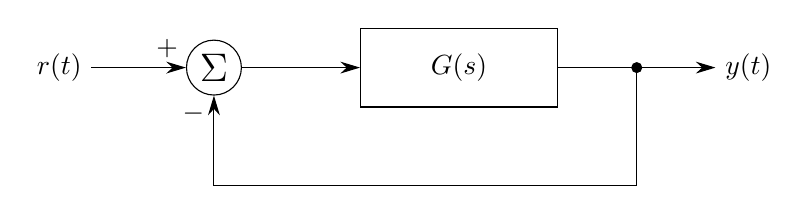
\begin{tikzpicture}[>={Stealth[length=2.5mm, width=1.5mm]}]
    % Nodes
    \node (rt) {$r(t)$};
    \node[draw, circle, right=1.2cm of rt, inner sep=2pt] (sum) {\Large $\Sigma$};
    \node[draw, rectangle, right=1.5cm of sum, minimum width=2.5cm, minimum height=1cm] (gs) {$G(s)$};
    \node[right=2cm of gs] (yt) {$y(t)$};
    \coordinate (branch) at ([xshift=1cm]gs.east);

    % Connections
    \draw[->] (rt) -- node[pos=0.8, above] {$+$} (sum);
    \draw[->] (sum) -- (gs);
    \draw[->] (gs) -- (yt);
    \draw[->] (branch) -- ++(0,-1.5cm) -| node[pos=0.9, left] {$-$} (sum.south);
    \fill (branch) circle (2pt);
\end{tikzpicture}

\vspace{0.2cm}
Fig. 1.1.124.1
\end{center}

\vspace{0.8cm}
\noindent For a unit step input $r(t)$, the steady state error in the output will be 

\vspace{0.3cm}
\noindent
\begin{tabular*}{\textwidth}{@{\extracolsep{\fill}} l l l l @{}}
    i) $0$ & ii) $1$ & iii) $2$ & iv) $\infty$
\end{tabular*}
\end{frame}

% ==========================================
% SECTION I: FUNDAMENTALS & INTRO
% ==========================================
\section{Resolving the System}


\begin{frame}{State-Space Representation}
        State-Space simplifies high-order DEs for representing systems by breaking any $n$-th order equation into $n$ coupled 1st-order equations:
        \begin{align}
            \dot{\vec{x}}(t) &= \vec{A}\vec{x}(t) + \vec{B}u(t) \quad \text{(State Equation)} \\
            y(t) &= \vec{C}\vec{x}(t) \quad \text{(Output Equation)}
        \end{align}
%        \item \textbf{Intuition:}
%        \begin{itemize}
%            \item $\vec{x}(t)$: The system's "memory" or internal states (e.g., position, velocity).
%            \item $\vec{A}$: The system matrix. It dictates how the states naturally interact.
%            \item $\vec{B}$: The input matrix. How the outside world's input $u(t)$ "pushes" the states.
%            \item $\vec{C}$: The output matrix. Which internal states can we actually measure?
%        \end{itemize}
\end{frame}
\begin{frame}{Deriving the System ODE}
        By expanding the matrices into algebraic equations:
        \begin{align}
            \myvec{\dot{x}_1 \\ \dot{x}_2} &= \myvec{0 & 1 \\ 0 & -2}\myvec{x_1 \\ x_2} + \myvec{0 \\ 1}u \implies \begin{cases} \dot{x}_1 = x_2 \\ \dot{x}_2 = -2x_2 + u \end{cases} \\
                                           &\text{Applying output equation:} \\
            y &= x_1 \\
            \dot{y} &= \dot{x}_1 = x_2 \\
            \ddot{y} &= \dot{x}_2 \\
            \implies \ddot{y} &= -2x_2 + u \\
            \ddot{y} &= -2\dot{y} + u \implies \ddot{y} + 2\dot{y} = u(t)
        \end{align}
\end{frame}

\begin{frame}{Deriving Transfer Function}
    \begin{itemize}
        \item Frequency-domain transfer function is given by $G(s) = \frac{Y(s)}{U(s)}$
        \item Apply the Laplace transform to the state equation, assuming zero initial conditions ($\vec{x}(0) = 0$):
        \begin{align}
            \mathcal{L}\{\dot{\vec{x}}(t)\} &= \mathcal{L}\{\vec{A}\vec{x}(t) + \vec{B}u(t)\} \\
            s\vec{X}(s) &= \vec{A}\vec{X}(s) + \vec{B}U(s) \\
            \implies (s\vec{I} - \vec{A})\vec{X}(s) = \vec{B}U(s) &\implies \vec{X}(s) = (s\vec{I} - \vec{A})^{-1}\vec{B}U(s) \\
            \implies Y(s) = \vec{C}(s\vec{I} - \vec{A})^{-1}\vec{B}U(s) &\implies G(s) = \vec{C}(s\vec{I} - \vec{A})^{-1}\vec{B}
        \end{align}
    \end{itemize}
\end{frame}

% ==========================================
% SECTION II: PART A - TRANSFER FUNCTION
% ==========================================
\section{Part A: Solving for $G(s)$}

\begin{frame}{Direct Resolution}
    \begin{itemize}
        \item Using the derived formula $G(s) = \vec{C}(s\vec{I} - \vec{A})^{-1}\vec{B}$.
        \item First, compute Resolvent Matrix: $(s\vec{I} - \vec{A})^{-1}$:
        \begin{align}
            s\vec{I} - \vec{A} &= \myvec{ s & -1 \\ 0 & s+2 } \\
            (s\vec{I} - \vec{A})^{-1} &= \frac{1}{s(s+2)} \myvec{ s+2 & 1 \\ 0 & s }
        \end{align}
        \item Multiplying by the input and output vectors:
        \begin{align}
            G(s) &= \myvec{ 1 & 0 } \left[ \frac{1}{s(s+2)} \myvec{ s+2 & 1 \\ 0 & s } \right] \myvec{ 0 \\ 1 } = \frac{1}{s(s+2)}
        \end{align}
    \end{itemize}
\end{frame}

\begin{frame}{Modal Analysis}
    \begin{itemize}
        \item Looking at $\vec{A} = \myvec{0 & 1 \\ 0 & -2}$. The top row gives $\dot{x}_1 = x_2$. The states are coupled together, which is why direct matrix inversion can be tedious for large systems.
        \item Thus, we use Spectral Decomposition to find a new coordinate system where the states are independent. This breaks the complex system into simple, parallel first-order filters.
        \item We do this by finding the eigenvalues and eigenvectors of $\vec{A}$.
        \begin{align}
            \det(\lambda\vec{I} - \vec{A}) = \lambda(\lambda + 2) = 0 \implies \lambda_1 = 0, \lambda_2 = -2
        \end{align}
    \end{itemize}
\end{frame}

\begin{frame}{Modal Analysis}
    \begin{itemize}
        \item Using the eigenvectors, we construct the modal matrix $\vec{V}$ and its inverse $\vec{V}^{-1}$:
        \begin{align}
            \vec{V} = \myvec{ 1 & 1 \\ 0 & -2 }, \quad \vec{V}^{-1} = \myvec{ 1 & 0.5 \\ 0 & -0.5 }
        \end{align}
        \item We transform the system: $\vec{\Lambda} = \vec{V}^{-1}\vec{A}\vec{V}$, $\vec{B}_m = \vec{V}^{-1}\vec{B}$, $\vec{C}_m = \vec{C}\vec{V}$.
        \item The transformed matrix $\vec{\Lambda}$ is perfectly diagonal:
        \begin{align}
            \vec{\Lambda} &= \myvec{ 0 & 0 \\ 0 & -2 }, \quad \vec{B}_m = \myvec{ 0.5 \\ -0.5 }, \quad \vec{C}_m = \myvec{ 1 & 1 }
        \end{align}
        \item Because $\vec{\Lambda}$ is diagonal, $(s\vec{I} - \vec{\Lambda})^{-1}$ is simply the inverted diagonal entries:
        \begin{align}
            G(s) = \vec{C}_m(s\vec{I} - \vec{\Lambda})^{-1}\vec{B}_m = \frac{0.5}{s} - \frac{0.5}{s+2} = \frac{1}{s(s+2)}
        \end{align}
    \end{itemize}
\end{frame}

% ==========================================
% SECTION III: PART B - STEADY STATE ERROR
% ==========================================
\section{Part B: Steady-State Analysis}

\begin{frame}{Deriving the Closed-Loop Matrix ($\vec{A}_{cl}$)}
    \begin{itemize}
        \item Unity negative feedback means the input $u(t)$ is the difference between the reference $r(t)$ and output $y(t)$:
        \begin{align}
            u(t) &= r(t) - y(t) = r(t) - \vec{C}\vec{x}(t)
        \end{align}
        \item Substitute this back into the original state equation:
        \begin{align}
            \dot{\vec{x}}(t) &= \vec{A}\vec{x}(t) + \vec{B}(r(t) - \vec{C}\vec{x}(t)) \\
            \dot{\vec{x}}(t) &= (\vec{A} - \vec{B}\vec{C})\vec{x}(t) + \vec{B}r(t)
        \end{align}
        \item The new system dynamics are governed by $\vec{A}_{cl} = \vec{A} - \vec{B}\vec{C}$:
        \begin{align}
            \vec{A}_{cl} &= \myvec{ 0 & 1 \\ 0 & -2 } - \myvec{ 0 & 0 \\ 1 & 0 } = \myvec{ 0 & 1 \\ -1 & -2 }
        \end{align}
    \end{itemize}
\end{frame}

\begin{frame}{Equivalence of Time and Frequency Limits}
    \begin{itemize}
        \item To find the steady-state output $y_{ss}$, we can evaluate the system as $t \to \infty$ or as $s \to 0$. They are physically identical.
        \vspace{0.2cm}
        \item \textbf{Time Domain ($t \to \infty$):} The system settles, so velocity $\dot{\vec{x}} = \vec{0}$.
        \begin{align}
            \vec{0} &= \vec{A}_{cl}\vec{x}_{ss} + \vec{B}r_{ss} \implies \vec{x}_{ss} = -\vec{A}_{cl}^{-1}\vec{B}r_{ss} \\
            y_{ss} &= \vec{C}\vec{x}_{ss} = \left(-\vec{C}\vec{A}_{cl}^{-1}\vec{B}\right)r_{ss}
        \end{align}
        \vspace{0.2cm}
        \item \textbf{Frequency Domain ($s \to 0$):} DC Gain $H(0)$. Let $s=0$ in the closed-loop transfer function $H(s) = \vec{C}(s\vec{I} - \vec{A}_{cl})^{-1}\vec{B}$:
        \begin{align}
            H(0) &= -\vec{C}\vec{A}_{cl}^{-1}\vec{B} \implies y_{ss} = H(0)r_{ss}
        \end{align}
    \end{itemize}
\end{frame}

\begin{frame}{Calculating Steady-State Error ($e_{ss}$)}
    \begin{itemize}
        \item Calculate the unified DC gain factor, $-\vec{C}\vec{A}_{cl}^{-1}\vec{B}$:
        \begin{align}
            \vec{A}_{cl}^{-1} &= \frac{1}{(0)(-2)-(-1)(1)} \myvec{ -2 & -1 \\ 1 & 0 } = \myvec{ -2 & -1 \\ 1 & 0 } \\
            H(0) &= -\myvec{ 1 & 0 } \myvec{ -2 & -1 \\ 1 & 0 } \myvec{ 0 \\ 1 } = -(-1) = 1
        \end{align}
        %\item \textbf{Conclusion:} A DC gain of 1 means the system perfectly replicates a constant input. 
        \item For a unit step input ($r_{ss} = 1$), the output is $y_{ss} = 1 \times 1 = 1$.
        \item The error is defined as $e_{ss} = \text{Input} - \text{Output}$:
        \begin{align}
            e_{ss} = 1 - 1 = 0
        \end{align}
    \end{itemize}
\end{frame}

% ==========================================
% SECTION IV: PART C - SIMULATION & DISCRETIZATION
% ==========================================
\section{Part C: Simulation \& Discretization}

\begin{frame}{Transient Analysis: Critical Damping}
    \begin{itemize}
        \item Before simulating the transition to steady-state, the roots of the closed-loop matrix $\vec{A}_{cl}$ are given by:
        \begin{align}
            \det(\lambda\vec{I} - \vec{A}_{cl}) &= \lambda^2 + 2\lambda + 1 = (\lambda + 1)^2 = 0
        \end{align}
        \item The system has a repeated real root at $\lambda = -1$.
        \item Comparing with the standard $2^{\text{nd}}$ order DE $s^2 + 2\zeta\omega_n s + \omega_n^2 = 0$:
        \begin{align}
            \omega_n^2 = 1 \implies \omega_n = 1 \\
            2\zeta\omega_n = 2 \implies \zeta = 1
        \end{align}
        \item $\zeta = 1$ dictates the system is critically damped.
    \end{itemize}
\end{frame}

\begin{frame}{Method 1: Numerical Integration via RK4}
    \begin{itemize}
        \item At step $t_n$ with size $h$, RK4 averages four intermediate slopes:
        \begin{align}
            \vec{k}_1 &= \vec{A}_{cl}\vec{x}_n + \vec{B}r(t_n) \\
            \vec{k}_2 &= \vec{A}_{cl}\left(\vec{x}_n + \frac{h}{2}\vec{k}_1\right) + \vec{B}r\left(t_n + \frac{h}{2}\right) \\
            \vec{k}_3 &= \vec{A}_{cl}\left(\vec{x}_n + \frac{h}{2}\vec{k}_2\right) + \vec{B}r\left(t_n + \frac{h}{2}\right) \\
            \vec{k}_4 &= \vec{A}_{cl}(\vec{x}_n + h\vec{k}_3) + \vec{B}r(t_n + h)
        \end{align}
        \item State update: $\vec{x}_{n+1} = \vec{x}_n + \frac{h}{6}(\vec{k}_1 + 2\vec{k}_2 + 2\vec{k}_3 + \vec{k}_4)$.
        \item However, this approximation has $\mathcal{O}(h^5)$ error. RK4 is normally used when shape of graph is unknown, for LTI system it's redundant.
    \end{itemize}
\end{frame}

\begin{frame}{Method 2: Deriving Discrete Difference Equation}
    \begin{itemize}
        \item Instead of guessing the slope, we start with the exact analytical continuous solution to $\dot{\vec{x}}(t) = \vec{A}_{cl}\vec{x}(t) + \vec{B}r(t)$:
        \begin{align}
            \vec{x}(t) = e^{\vec{A}_{cl}(t-t_0)}\vec{x}(t_0) + \int_{t_0}^{t} e^{\vec{A}_{cl}(t-\tau)}\vec{B}r(\tau) d\tau
        \end{align}
        \item To compute the next digital sample $\vec{x}[k+1]$ at time $t = (k+1)T_s$ using the current sample $\vec{x}[k]$ at $t_0 = kT_s$, we substitute these times into the integral:
        \begin{align}
            \vec{x}((k+1)T_s) = e^{\vec{A}_{cl}T_s}\vec{x}(kT_s) + \int_{kT_s}^{(k+1)T_s} e^{\vec{A}_{cl}((k+1)T_s-\tau)}\vec{B}r(\tau) d\tau
        \end{align}
    \end{itemize}
\end{frame}

\begin{frame}{Method 2: Deriving Discrete Difference Equation}
    \begin{itemize}
        \item Usually, the input $r(\tau)$ is held constant during the sample interval. So, $r(\tau) = r[k]$.
        \item Because $r[k]$ is constant, we can pull it completely out of the integral. 
        \item Let $\sigma = (k+1)T_s - \tau$:
        \begin{align}
            \vec{x}[k+1] &= \underbrace{\left(e^{\vec{A}_{cl}T_s}\right)}_{\vec{\Phi}_d} \vec{x}[k] + \underbrace{\left(\int_0^{T_s} e^{\vec{A}_{cl}\sigma} d\sigma \vec{B}\right)}_{\vec{\Gamma}_d} r[k]
        \end{align}
        \item Thus the exact discrete difference equation is $\vec{x}[k+1] = \vec{\Phi}_d \vec{x}[k] + \vec{\Gamma}_d r[k]$.
    \end{itemize}
\end{frame}

\begin{frame}{Method 2: Solving the Matrix Exponential}
    \begin{itemize}
        \item To use this exact mapping, we must evaluate $\vec{\Phi}_d = e^{\vec{A}_{cl}T_s}$. 
        \item Because our system is critically damped (repeated eigenvalue $\lambda=-1$), the \textbf{Cayley-Hamilton Theorem} allows us to evaluate the infinite Taylor series of the exponential exactly as a simple linear polynomial:
        \begin{align}
            e^{\vec{A}_{cl}t} &= e^{\lambda t} \left( \vec{I} + (\vec{A}_{cl} - \lambda\vec{I})t \right) \\
            \vec{\Phi}_d &= e^{-T_s} \myvec{ 1+T_s & T_s \\ -T_s & 1-T_s }
        \end{align}
        \item Using these exact discrete matrices ensures that our step-by-step software simulations will flawlessly mimic the physical analog reality without any integration drift.
    \end{itemize}
\end{frame}

\section{Python Codes}
\begin{frame}[fragile,allowframebreaks]{Python Implementation}
    \lstinputlisting[basicstyle=\scriptsize\ttfamily]{../codes/plot.py}
\end{frame}
% ==========================================
% SECTION V: SIMULATION RESULTS
% ==========================================
\section{Simulation Results}
\begin{frame}{Sympy Verification}
    \begin{itemize}
        \item Sympy confirms all of the expressions we derived. Computer algebra systems are extremely cool.
    \end{itemize}
    \vspace{0.3cm}
    \begin{figure}[h]
        \centering
        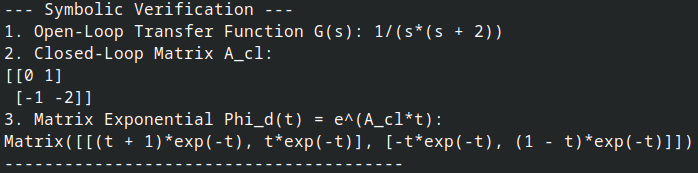
\includegraphics[width=0.95\textwidth]{../figs/fig0_sympy_verification.png}
    \end{figure}
\end{frame}
\begin{frame}{Simulation: Exact Discrete Method}
    \begin{itemize}
        \item Using our derived $\mathbf{\Phi}_d$ and $\mathbf{\Gamma}_d$, the digital simulation lands precisely on the continuous analytical curve at every sample instant ($T_s = 0.5$s).
    \end{itemize}
    \vspace{-0.2cm}
    \begin{figure}[h]
        \centering
        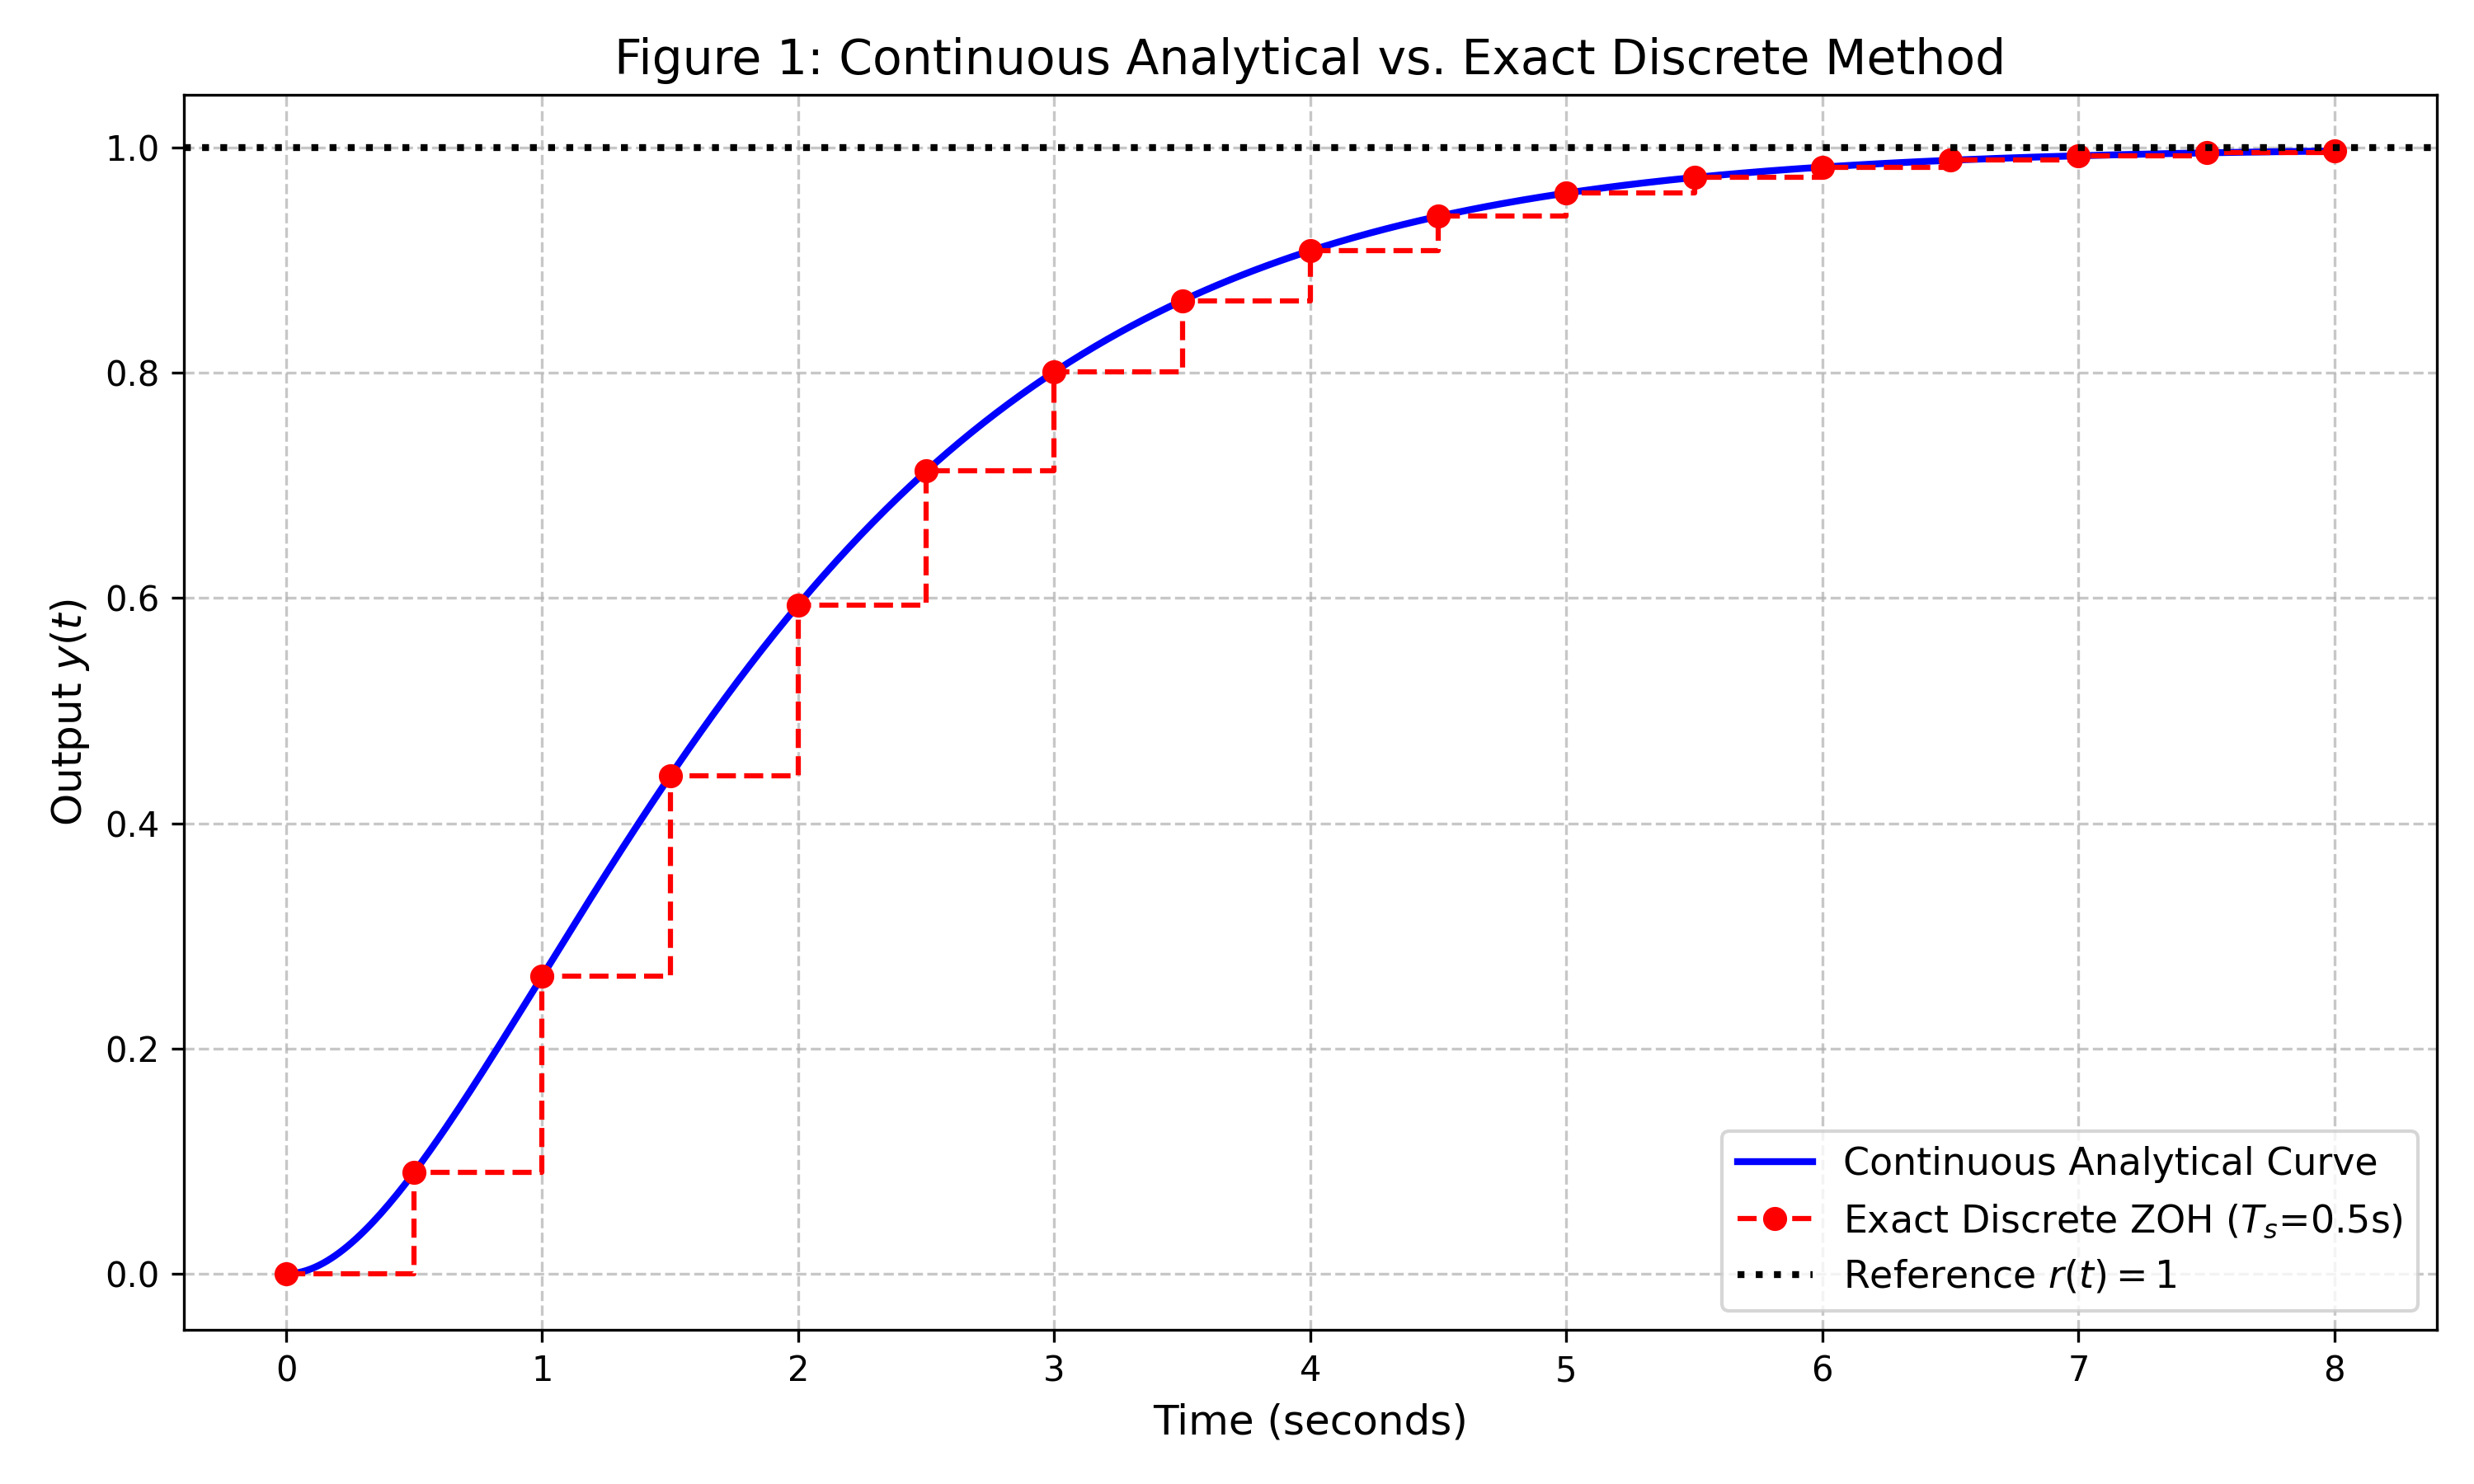
\includegraphics[width=0.85\textwidth]{../figs/fig1_exact_discrete.png}
    \end{figure}
\end{frame}

\begin{frame}{Simulation: RK4 Integration Approximation}
    \begin{itemize}
        \item Using the 4th-Order Runge-Kutta method with the same step size ($h = 0.5$s).
        \item On a macro scale, numerical integration appears to track the system perfectly toward the steady-state of $1$.
    \end{itemize}
    \vspace{-0.2cm}
    \begin{figure}[h]
        \centering
        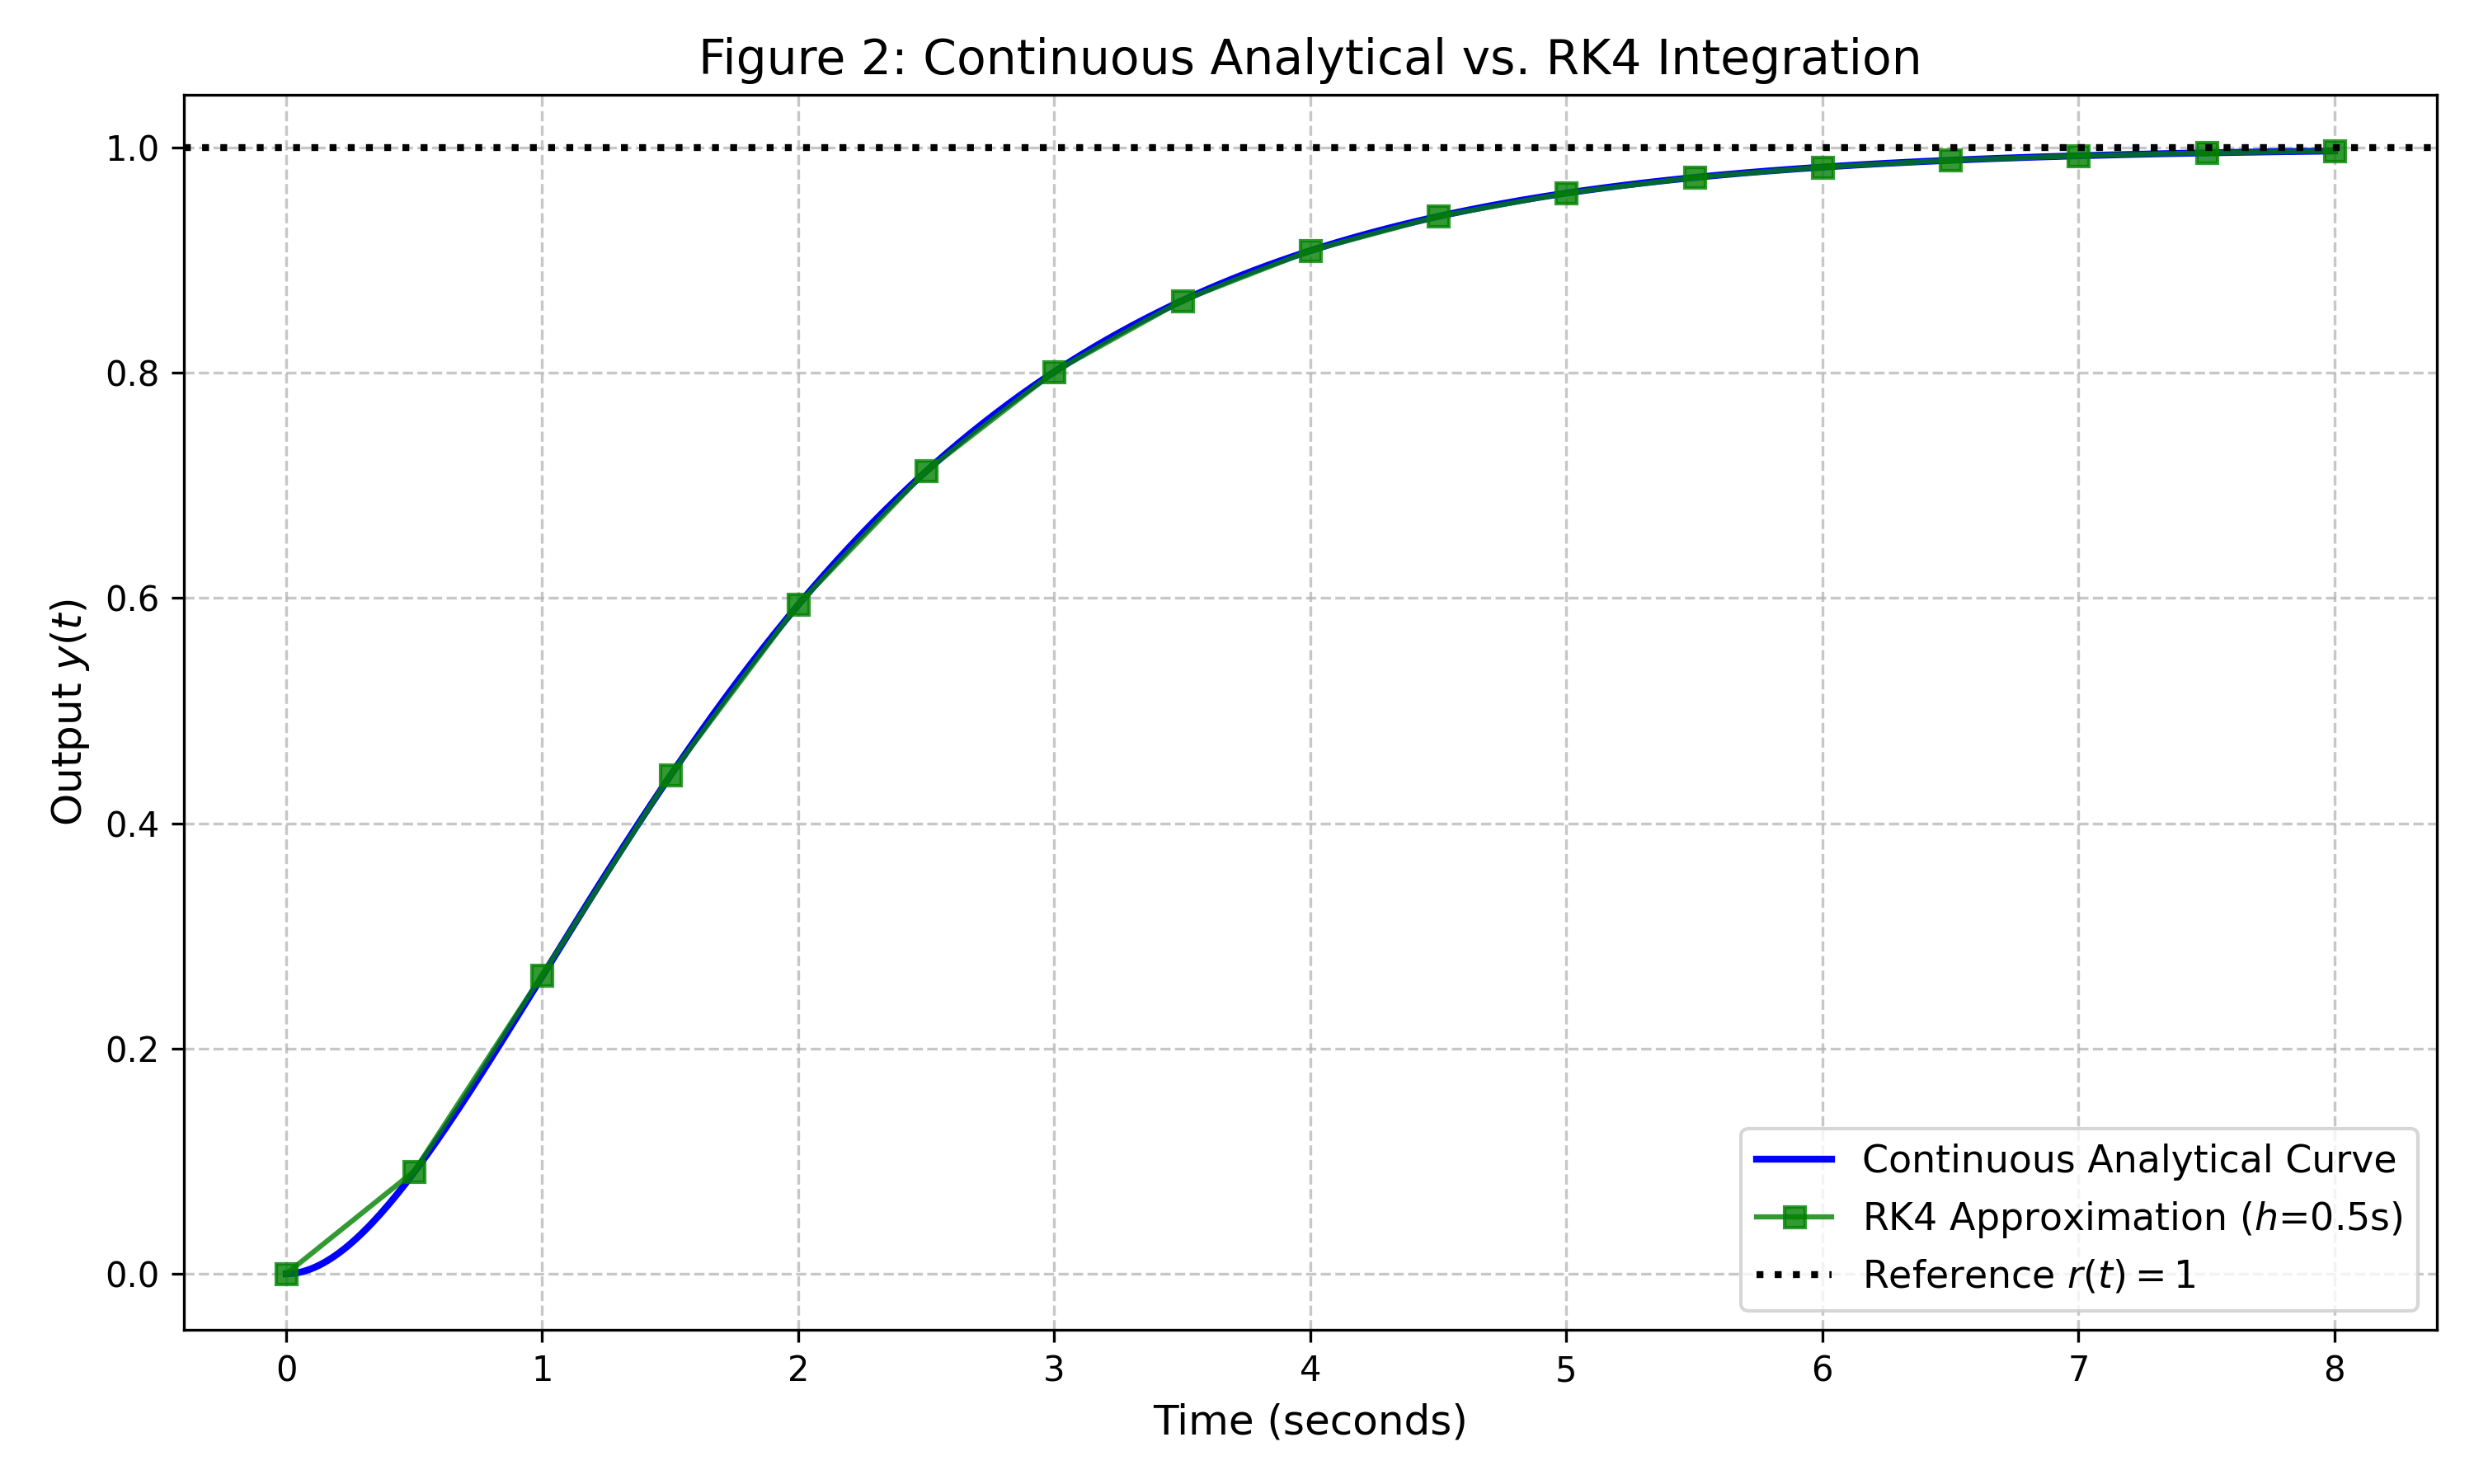
\includegraphics[width=0.85\textwidth]{../figs/fig2_rk4_comparison.png}
    \end{figure}
\end{frame}

\begin{frame}{Analysis at a Point}
    \begin{itemize}
        \item Zooming in precisely at $t = 1.5$s exposes the underlying geometry.
        \item Because RK4 is approximating the slope rather than using the exact analytical mapping, it misses the true curve.
        \item The exact discrete method computes the state flawlessly.
    \end{itemize}
    \vspace{-0.2cm}
    \begin{figure}[h]
        \centering
        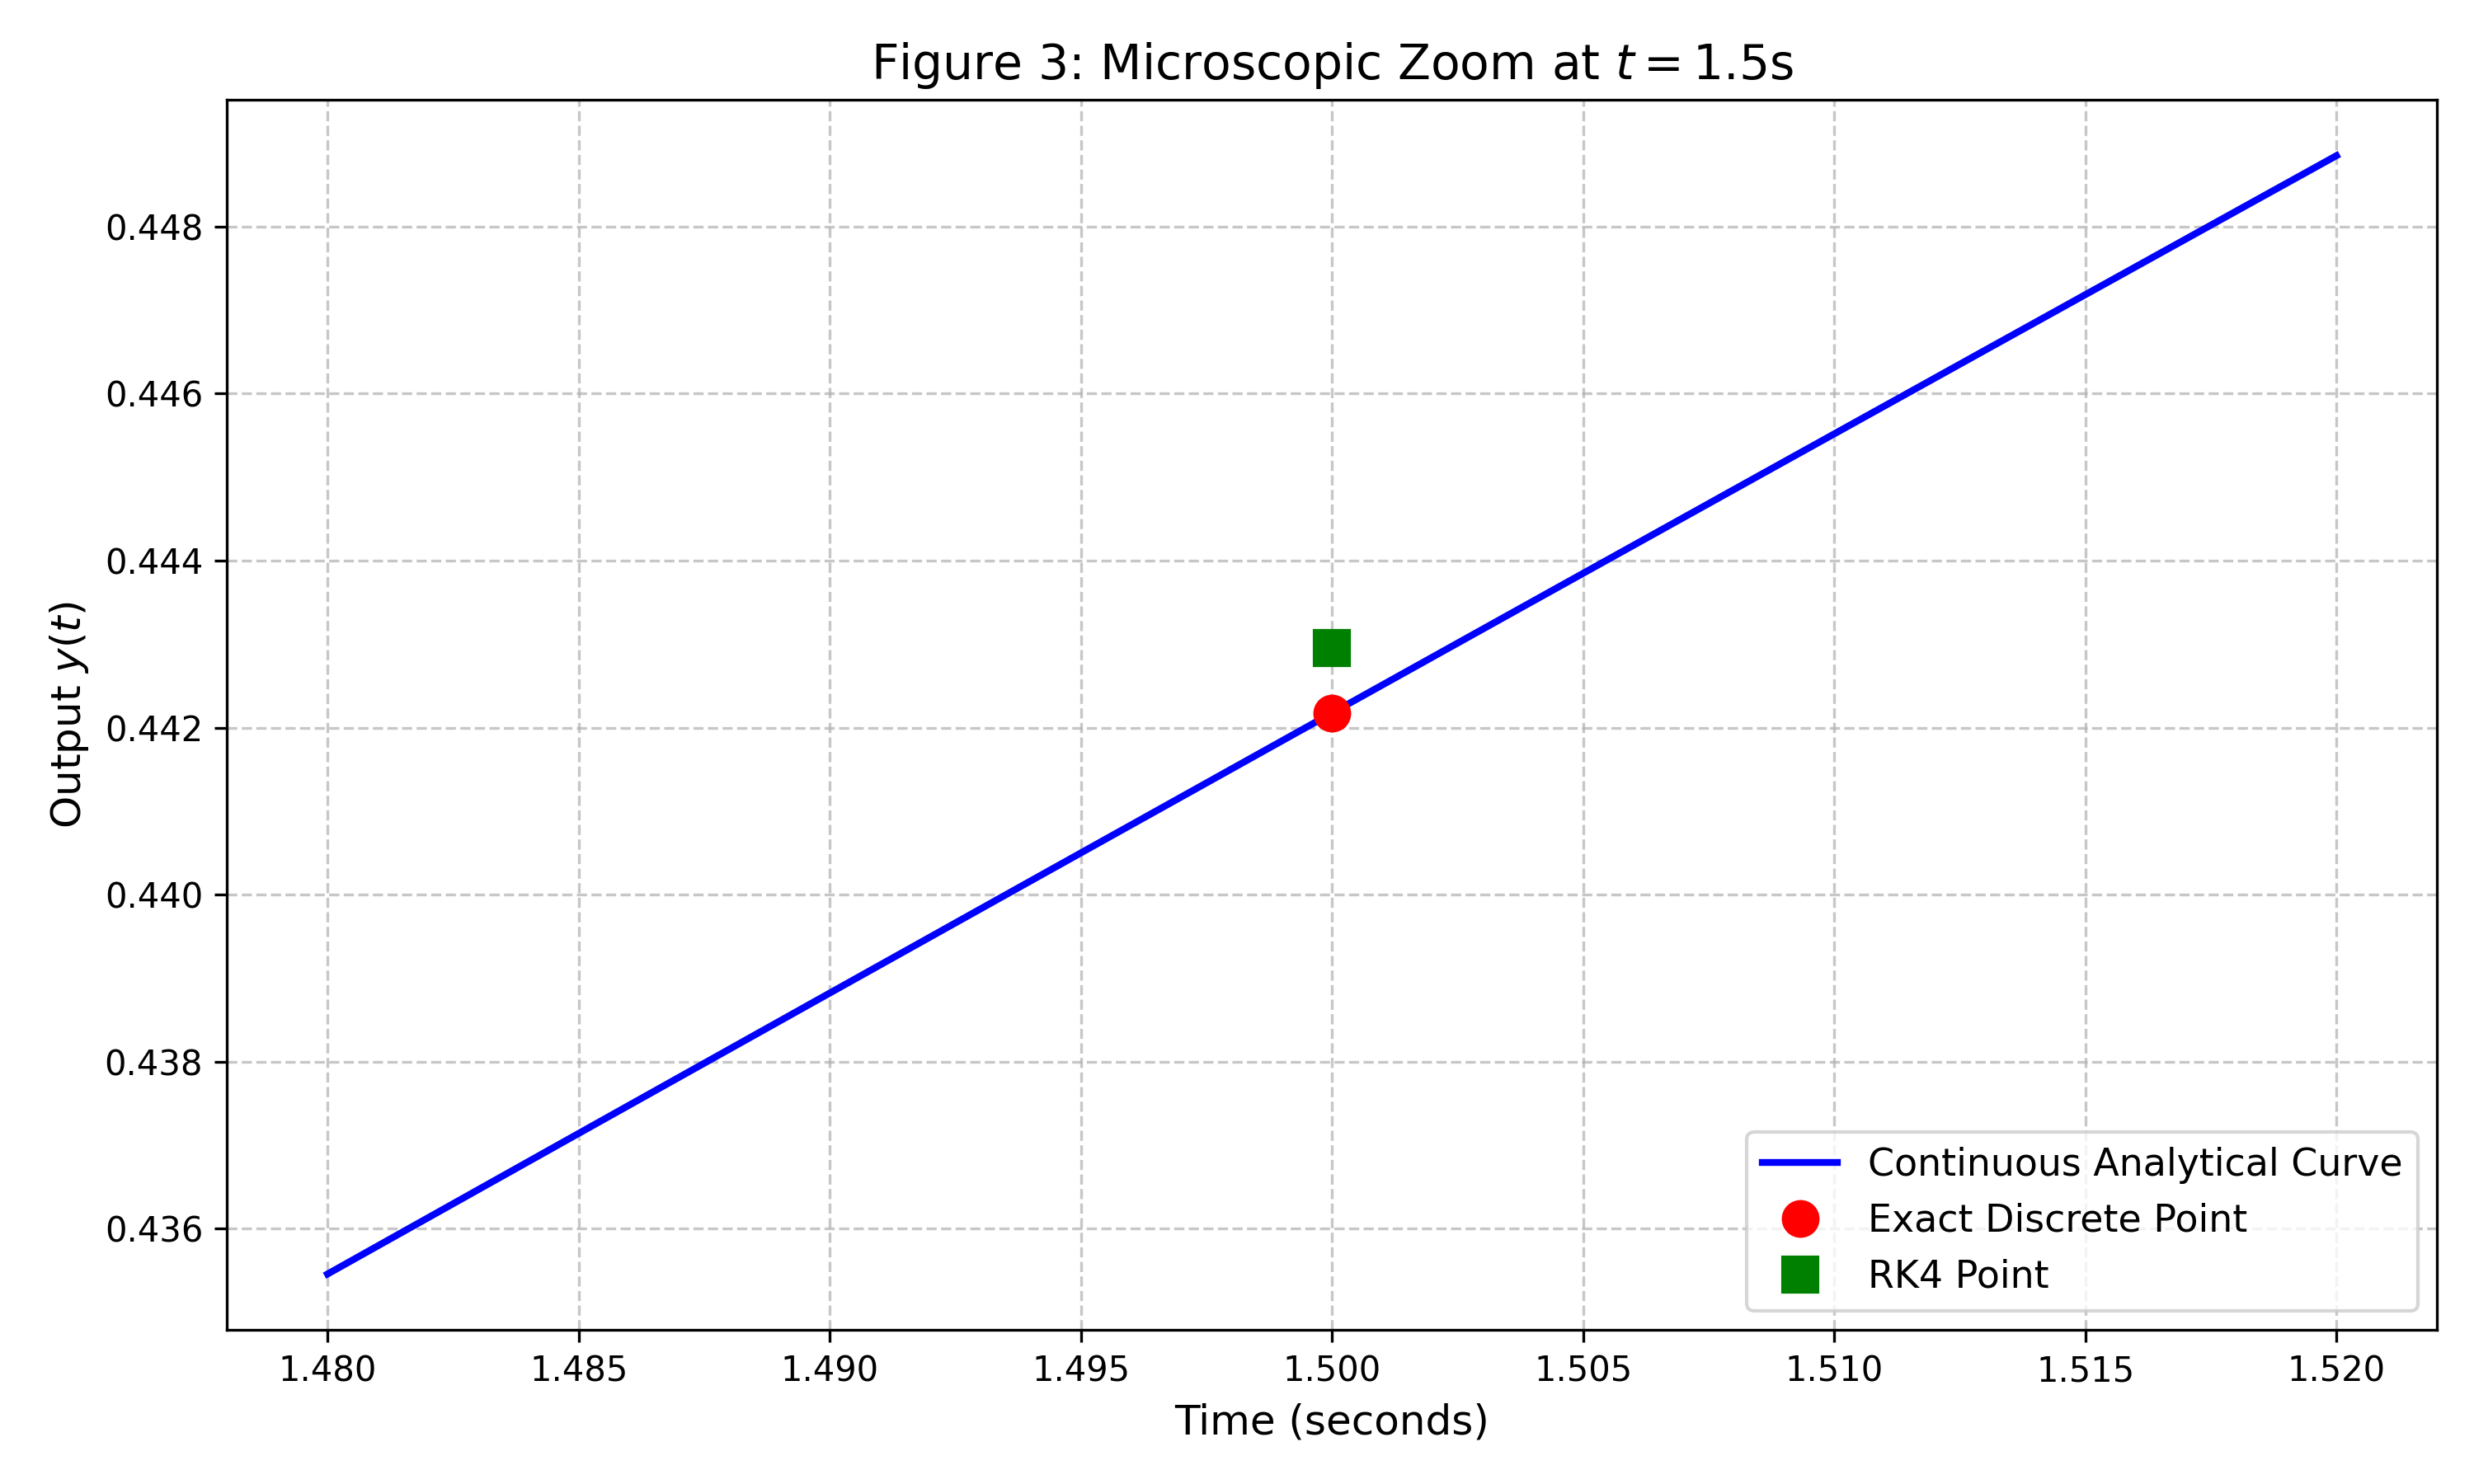
\includegraphics[width=0.85\textwidth]{../figs/fig3_zoomed.png}
    \end{figure}
\end{frame}

\begin{frame}{Error Analysis}
    \begin{itemize}
        \item Plotting the absolute error $|y_{true} - y_{sim}|$ on a logarithmic scale.
        \item RK4 produces an error hovering between $10^{-3}$ and $10^{-5}$.
        \item The Exact Discrete formulation's error is strictly bounded by IEEE 754 float limitations ($\sim 10^{-15}$), making it mathematically exact.
    \end{itemize}
    \vspace{-0.2cm}
    \begin{figure}[h]
        \centering
        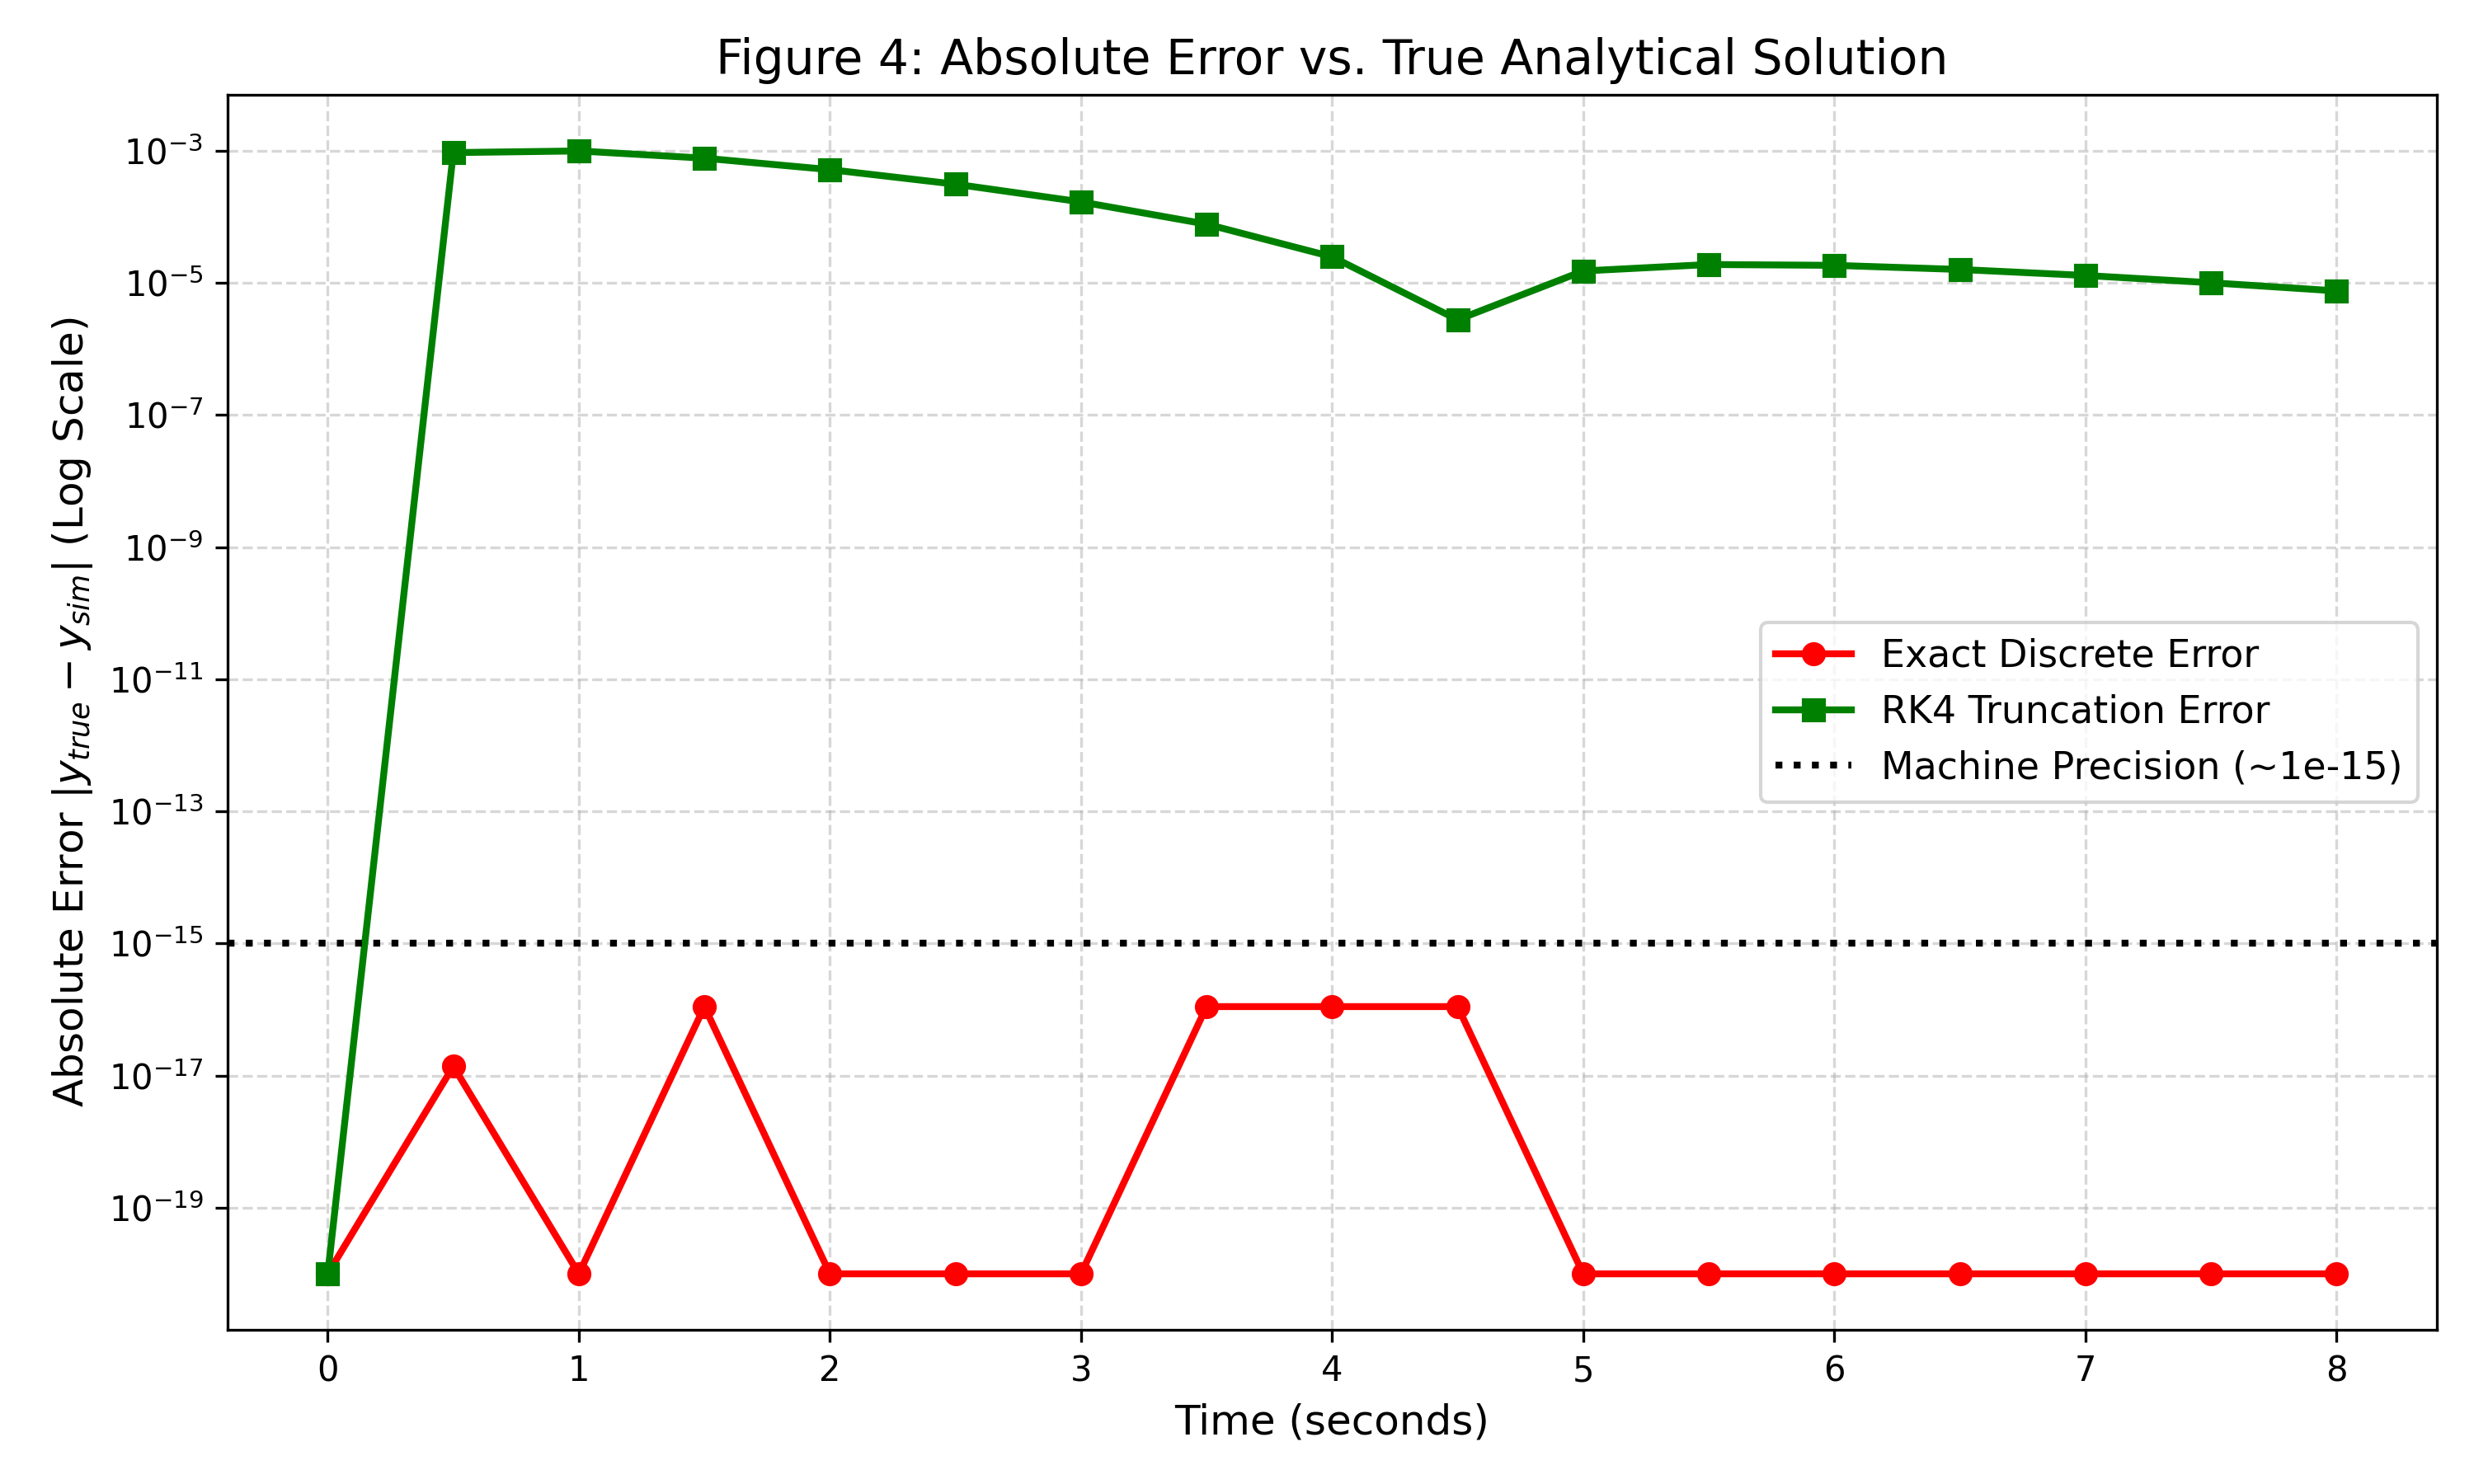
\includegraphics[width=0.85\textwidth]{../figs/fig4_error_log.png}
    \end{figure}
\end{frame}
\end{document}
